%
% File: chap01.tex
% Author: Victor F. Brena-Medina
% Description: Introduction chapter where the biology goes.
%
\let\textcircled=\pgftextcircled
\chapter{Introduction}
\label{chap:intro}
\vspace{-0.2 cm}

\section{Motivation}

\paragraph{}

With advancements in digital VLSI, chips which once could never be imagined can be fabricated. Making a digital ASIC involves many rigorous steps with feedback among different steps. Therefore, it is only human to expect several iterations of architecture, circuit and layout design. Even though ASICS produced in bulk are quite cheap, test ASICs that need to be fabricated while prototyping are very costly. FPGAs solve this issue by providing a fabric to test any digital circuit for functionality. 

\begin{figure}[h]
\centering
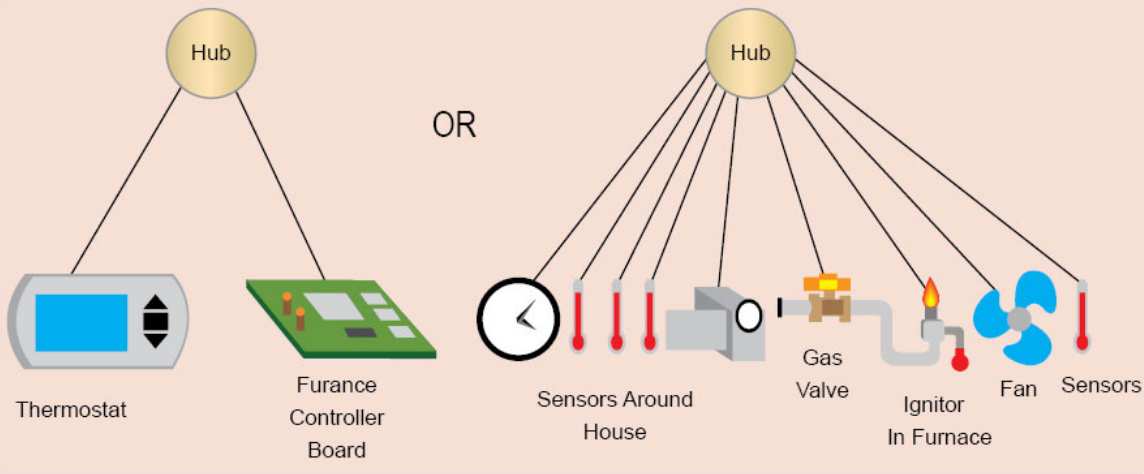
\includegraphics[width=0.9\linewidth]{FPGA_application_in_IOT_and_smart_solutions.png} 
\caption{Small FPGA hubs in smart-home solutions}
\label{fig:Figure}
\end{figure}

FPGAs work on the simple principles of boolean algebra and the use of flip-flops to implement state machines. Apart from facilitating cheap prototyping, FPGAs can also be used by itself in a product eliminating the need to incur the cost of ASIC design and fabrication at the cost of some granularity and overheads. This is a particularly attractive option for modest digital circuits or when you don't have enough input capital. ASICs have been shown to be two or three orders of magnitude better than general purpose processors for some applications. FPGAs can come in handy to reap a big part of these benefits with minimal input capital. Therefore, FPGAs are also popular as accelerators these days. In many digital systems, a very minimal FPGA is required to implement a modest logic like interfacing etc(See fig. 1.1). But even the smallest micro-controllers or FPGAs in the market(See fig. 1.2) are an overkill for such applications. Also, not many FPGA projects are completely open-source.

\begin{figure}[h]
\centering
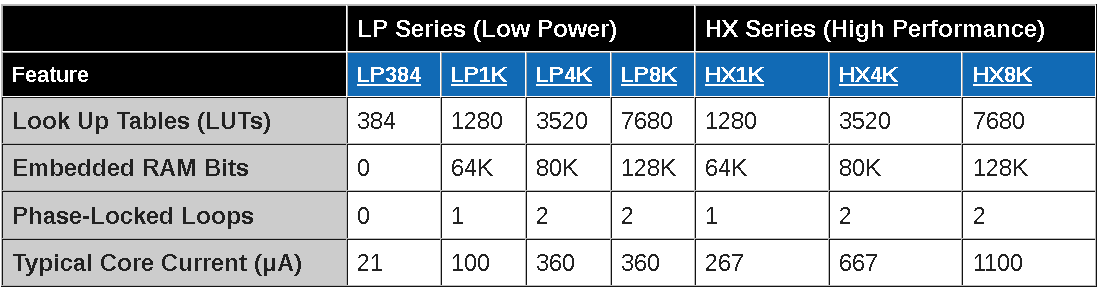
\includegraphics[width=0.9\linewidth]{lattice_tiny_family.png}
\caption{Lattice's family of miniature FPGAs[1]}
\label{fig:Figure}
\end{figure}

\begin{figure}[h]
\centering
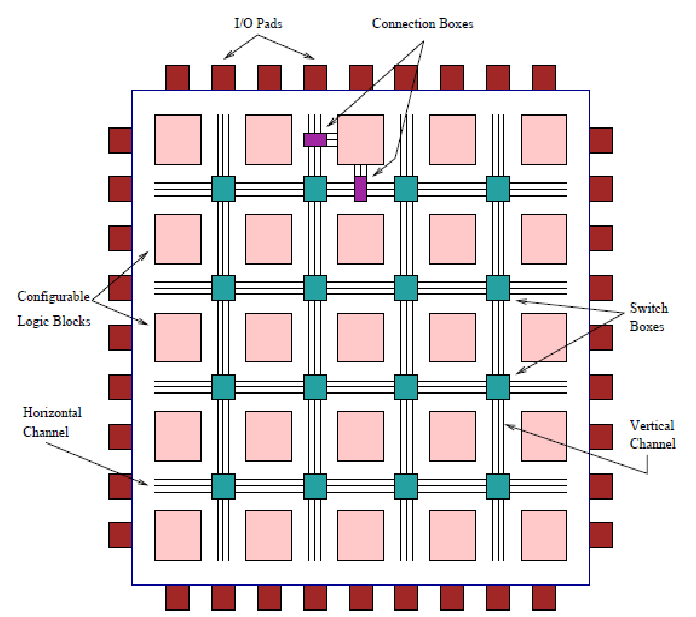
\includegraphics[width=0.6\textwidth]{Island-style.png}
\caption{Island-Style FPGA architecture}
\label{fig:Figure}
\end{figure}
Similarly, small and standard digital ASICs have overkill specifications for most use cases and thus a tiny FPGAs can emulate these ASICs quite comfortably. Island-style FPGAs are the most common with small LUTs(Look Up Tables) interconnected together with a mesh of programmable routing. 

We wish to develop a small island-style FPGA starting from scratch and my work tackles with the architectural-level design of the same. We first theoretically study the island-style FPGA in the light of SCL-180nm and derive useful results for the architecture of the FPGA. Furthermore, we have developed and tested(at schematic level) an 8X8 LUT island-style FPGA in SCL-180nm technology node.


\section{Previous Work}

\paragraph{}

Jonathan Rose[2] has done some work on architecting FPGAs. He first develops concepts of island-style FPGAs and then demonstrates different routing methods. He further provides a software tool to automate the layout generation of an FPGA by iteratively placing tiles of a CLB and Switch Matrix. This tool isnot compatible with modern PDKs and the tool isn't even available publically. Only a final netlist of their FPGA is provided which is not easy to scale or modify. 
[3] analyzes various parameters of an island-style FPGA architecture from theoretical derivations of area and delay but the models are approximate. The various area models used in the derivations are shown in Fig. 1.4. Equations 1.1 to 1.4 give approximations of total area required to layout an FPGA using these approximations. 

\begin{figure}[h]
\centering
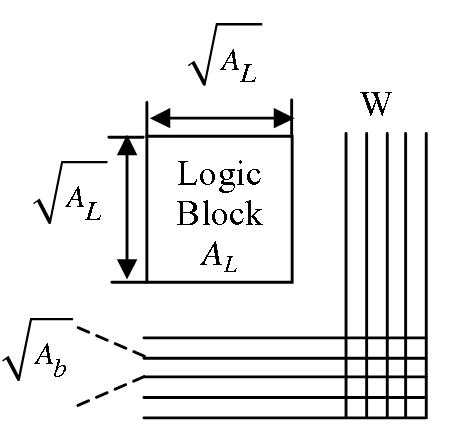
\includegraphics[width=0.3\linewidth]{area_model.png}
\caption{Area model used in [3]}
\label{fig:Figure}
\end{figure}

\begin{equation}
A_{Tile} = A_L + A_R
\end{equation}
\begin{equation}
A_L^K = A_b\cdot2^K + A_f
\end{equation}
\begin{equation}
A_R^K = A_b{\cdot}W_K^2 + 2\cdot\sqrt{A_b}\cdot\sqrt{A_L^K}{\cdot}W_K
\end{equation}
\begin{equation}
A_{Total}^K = A_{Tile}^K{\cdot}N_K = {(\sqrt{A_b}{\cdot}W_K + \sqrt{A_L^K})}^2{\cdot}N_K
\end{equation}

$A_{Tile}$ : Area of a single tile \hfill
$A_L$ : Area of Logic Block per tile \hfill
$A_R$ : Area of Routing per tile \hfill
$A_b$ : Area of an SRAM cell \hfill
$K$ : Number of Inputs to one CLB \hfill
$N_K$ : Number of tile required with K-size CLBs \hfill

\begin{figure}[h]
\centering
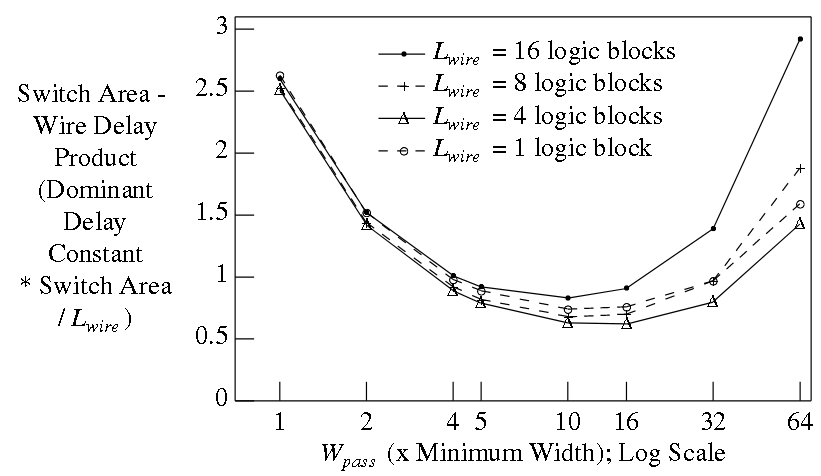
\includegraphics[width=0.9\linewidth]{previous_work.png}
\caption{Sizing pass transistors of the switch matrices[5]}
\label{fig:Figure}
\end{figure}

The FPGA research community has developed the VTR Project[4]. VTR(Verilog to Routing) is a tool chain which facilitates FPGA architecture research. The tool needs a description of the FPGA architecture in a special pre-defined XML format along with the Verilog file which is to be implemented on the FPGA. The tool will first determine the grid size and routing width needed to implement the circuit and then perform coarse and fine grained routing to produce a netlist. This tool is not very well supported in the schematic level circuit simulation softwares as well as layout tools. 

[5] proposes methodologies to size interconnect circuits as shown in Fig. 1.5 but does not consider the effect of CLB circuit on the sizing by assuming a buffer in between which limits it to a first hand approximation. We use these suggested values as a starting point in the project.

\section{Problem Definition}

\paragraph{}

The aim of this thesis is to architect a minimal Island-Style FPGA in SCL-180 nm technology node and test its functionality at schematic level using Cadence Virtuoso. The steps taken in this regard are as follows:
\begin{itemize}
  \item Understanding working of Island-Style FPGAs
  \item Deciding on the CLB
  \item Deciding on the Switch Matrix and I/O Block
  \item Deciding on the size of CLB Grid
  \item Designing the programmability of the FPGA
  \item Designing the address decoders
  \item Designing the schematic in Virtuoso
  \item Testing the circuit for functionality in virtuoso
\end{itemize}

\section{Contributions}
\paragraph{}
The objective of this thesis is to architect an Island-Style FPGA through various smaller steps as explained above. In designing this architecture and schematic, various tools/scripts have been prepared for automate schematic generation, stimulus generation, pipeline to program the FPGA schematic with a bitstream in spectre, etc. These contributions will be discussed in subsequesnt chapters.

\section{Thesis Organization}

\begin{itemize}
  \item \textbf{Chapter 1} gives an introduction to Island-Style FPGAs and the need for developing an open-source flow for minimal FPGA design.

  \item \textbf{Chapter 2} discusses the CLB design in detail along with involved architectural choices

  \item \textbf{Chapter 3} discusses the design of Switch Matrix 

  \item \textbf{Chapter 4} discusses the design of I/O Block

  \item \textbf{Chapter 5} discusses the programmability of the FPGA

  \item \textbf{Chapter 6} discusses the complete system level design of an 8x8 FPGA along with simulations

  \item \textbf{Chapter 7} Conclusion
\end{itemize}

